%%
% Please see https://bitbucket.org/rivanvx/beamer/wiki/Home for obtaining beamer.
%%
%\documentclass[11pt,aspectratio=169]{beamer}
%\documentclass[11pt,aspectratio=169,xcolor={dvipsnames}]{beamer}

\documentclass[11pt,aspectratio=169,xcolor={dvipsnames},hyperref={pdftex,pdfpagemode=UseNone,hidelinks,pdfdisplaydoctitle=true},usepdftitle=false]{beamer}
\usepackage{presentation}


\title{Lecture 11: Financial Frictions in the Long Run}
\author{Juan Herre\~{n}o\\UCSD}
\date{2026}

% Enter presentation title to populate PDF metadata:
\newcommand{\Cov}{\text{Cov}_\lambda}
\newcommand{\El}{\mathbb{E}_\lambda}
\newcommand{\mm}{\text{{\fontfamily{qzc}\selectfont m}}}
\usepackage{cancel}
\usepackage{booktabs}
\begin{document}

\maketitle


\begin{frame}{Motivation}
\begin{itemize}
\item Large dispersion in MPKs in developing countries (Hsieh and Klenow, 2009)
\begin{itemize}
\item Capital does not flow to the most productive hands
\end{itemize}
\item Large income differences across countries 
\begin{itemize}
\item Capital does not flow from rich to poor countries
\end{itemize}
\item Work in development suggests a large role for financial market imperfections ( Banerjee and Newman, 1993; Piketty, 1997; Aghion and Bolton, 1997; Banerjee and Duflo, 2005; ...)
\end{itemize}

We will follow Moll (2014).
\end{frame}


\begin{frame}{Simple Framework}
\begin{itemize}
\item Start with a static model, firms have Cobb-Douglas production functions with CRS
\[y_j = \left(z_j k_j\right)^{\alpha} l_j^{1-\alpha} \]
\item Financial constraint: May rent capital up to a multiple of their wealth
\[k_j < \lambda a_j \]
\item $\lambda \geq 1$ the extent of financial frictions. First best: $\lambda \rightarrow \infty$
\item Firms sell homogeneous goods, rent labor and capital in competitive markets
\[\Pi_j = y_j - w l_j - (r+\delta) k_j \]
\item Distribution of $a$ exogenous for now
\item $r$ and $w$ are endogenous objects, of course
\end{itemize}
\end{frame}

\begin{frame}{Simple Framework}
\begin{itemize}
\item Optimal labor demand is very simple
\[l_j = z_j k_j \left(\frac{w}{1-\alpha} \right)^{-1/\alpha}\]
\item Replace on the profit function
\[\Pi_j = (z_j \pi - r - \delta)k_j, \text{    with:  } \pi = \alpha\left(\frac{1-\alpha}{w}\right)^{(1-\alpha)/\alpha}\]
\item Profits are linear in $k$. Corner solution: Either $k_j = \lambda a_j$ or $k_j = 0$.
\item The marginal entrant has a productivity $\underline{z}$ such that
\[\Pi^*(\underline{z}) = 0 \]
\item Threshold is independent of $a$ and defined by $\underline{z}\pi = r + \delta$
\end{itemize}
\end{frame}

\begin{frame}{Intuition}
\begin{itemize}
\item Efficiency calls for allocating production to high MPK firms
\item Efficiency-improving to reallocate capital from low $z$ to high $z$ firms
\item Financial market imperfections prevent that to happen
\item Firms of wealthy owners with low $z$ may be larger than firms of poor owners with high $z$
\end{itemize}
\end{frame}


\begin{frame}{Simple Framework}
\begin{itemize}
\item Preview
\begin{itemize}
\item We can aggregate this economy from the bottom-up
\[Y = Z K^{\alpha} L^{1-\alpha}\]
\item Financial frictions aggregate to endogenous TFP losses
\item Intuition: In the first best, only entrepreneurs with the max $z$ operate their technology (CRS)
\item Away from the first best, there is negative selection of the marginal entrepreneur
\end{itemize}
\end{itemize}
\end{frame}

\begin{frame}{Steps for Aggregation}
\begin{itemize}
\item Define the share of wealth held by type $z$
\[\omega(z) = \frac{ \int_0^{\infty} a g(a,z) da}{\int a dG(a,z)}\]
\item And the CDF of wealth held by entrepreneurs of productivity less than $z$
\[\Omega(z) = \int_0^z \omega(x) dx\]
\item Market clearing condition in the capital market implies that
\[\int a dG(a,z) = \int k(a,z) dG(a,z)\]
\end{itemize}
\end{frame}

\begin{frame}{Steps for Aggregation}
\[\int a dG(a,z) = \int k(a,z) dG(a,z)\]
\begin{itemize}
\item Active entrepreneurs demand $\lambda a_j$, non-active entrepreneurs demand 0 capital. Implying that (homework)
\[1 = \lambda( 1 - \Omega(\underline{z}))\]
\item Given wealth shares (exogenous for now), pins down $\underline{z}$ as a function of $\lambda$.
\item If $\lambda$ is lower, then $\underline{z}$ lower as well:
\begin{itemize}
\item Share of wealth owned by non-active entrepreneurs decreases
\end{itemize}
\item The marginal entrant is less productive!
\end{itemize}
\end{frame}

%\begin{frame}
%$$K = \int_{\underline{z}}^{\bar{z}} \int_0^{\infty} \lambda a g(a,z) da dz$$
%$$1 = \lambda \int_{\underline{z}}^{\bar{z}} \omega(z) dz$$
%$$1 = \lambda (1- \int_{0}^{\underline{z}} \omega(z) dz)$$
%$$1 = \lambda (1-\Omega(\underline{z}))$$
%\end{frame}


\begin{frame}{Steps for Aggregation}
\begin{itemize}
\item Aggregate production is the integral of individual production
\[Y = \int_0^{\bar{z}} \int_0^{\infty} y(a,z) g(a,z) da dz\]
\item Can be written (become familiar with the math!)
\[Y = \left(\frac{1-\alpha}{w}\right)^{\frac{1-\alpha}{\alpha}} \lambda K \int_{\underline{z}}^{\bar{z}} z \omega(z) dz \]
\item Not a production function. $Y$ depends on input prices ($w$).
\end{itemize}
\end{frame}


\begin{frame}{Steps for Aggregation}
\[Y = \left(\frac{1-\alpha}{w}\right)^{\frac{1-\alpha}{\alpha}} \lambda K \int_{\underline{z}}^{\infty} z \omega(z) dz \]
\begin{itemize}
\item Use mkt clearing for labor (inelastic supply $L$)
\[L = \int \int l(a,z) dG(a,z)\]
\item Similar math to before (check the labor demand equation on slide 4)
\[L = \left(\frac{1-\alpha}{w}\right)^{\frac{1}{\alpha}} \lambda K  \int_{\underline{z}}^{\bar{z}} z \omega(z) dz\]
\item solve for $\left(\frac{1-\alpha}{w}\right)^{\frac{1}{\alpha}}$ and plug back into aggregate output
\[Y = \lambda^{\alpha} K^{\alpha} L^{1-\alpha} \left(\int_{\underline{z}}^{\bar{z}} z \omega(z) dz\right)^{\alpha}\]
\end{itemize}
\end{frame}

\begin{frame}{Steps for Aggregation}
\[Y = \lambda^{\alpha} K^{\alpha} L^{1-\alpha} \left(\int_{\underline{z}}^{\infty} z \omega(z) dz\right)^{\alpha}\]
\begin{itemize}
\item We are done. Improve the interpretation. Remember mkt clearing of $K$
\[1 = \lambda(1- \Omega(\underline{z}))\]
\item And by laws of conditional expectations
\[  \mathbb{E}_{\omega} \left[z| z> \underline{z} \right] = \frac{\left(\int_{\underline{z}}^{\infty} z \omega(z) dz\right)}{1-\Omega(\underline{z})} \]
\item Is the (wealth share-weighted) average productivity among active entrepreneurs
\[Y = ZK^{\alpha} L^{1-\alpha}\]
\item with $Z =  \mathbb{E}_{\omega} \left[z| z> \underline{z} \right]^{\alpha}$
\end{itemize}
\end{frame}


\begin{frame}{Lessons from the static model}
\[Y = ZK^{\alpha} L^{1-\alpha}\]
\[Z =  \mathbb{E}_{\omega} \left[z| z> \underline{z} \right]^{\alpha}\]

\begin{itemize}
\item We recovered your neoclassical growth model from 210A
\item But with an endogenous TFP
\item Starting from a continuum of heterogeneous firms with inequality
\item TFP depends on the distribution of technical productivity in the population
\item But also on allocative efficiency: are talented folks able to access the means of production?
\item Under financial frictions, it matters who ($z$) owns the wealth $a$.
\item Not in the first best. The financial market takes care of dictating the flow of funds
\end{itemize}

\end{frame}


\begin{frame}{Why does not capital flow to poorer countries?}
\begin{itemize}
\item Remember the free entry condition
\[\underline{z}\  \alpha\left(\frac{1-\alpha}{w}\right)^{(1-\alpha)/\alpha} = r + \delta\]
\item Use this useful intermediate step we derived
\[Y = \left(\frac{1-\alpha}{w}\right)^{\frac{1-\alpha}{\alpha}} \lambda K \int_{\underline{z}}^{\infty} z \omega(z) dz \]
\item Along with mkt clearing in $K$
\[r + \delta = \alpha \frac{\underline{z}}{\mathbb{E}_{\omega} \left[z| z> \underline{z} \right]} Z K^{\alpha-1}L^{1-\alpha} \]
\item Note that $\frac{\underline{z}}{\mathbb{E}_{\omega} \left[z| z> \underline{z} \right]} \in [0,1]$
\end{itemize}
\end{frame}


\begin{frame}{Why does not capital flow to poorer countries?}
\[r + \delta =\alpha \left ( \frac{\underline{z}}{\mathbb{E}_{\omega} \left[z| z> \underline{z} \right]} \right) Z K^{\alpha-1}L^{1-\alpha}\]
\begin{itemize}
\item If we forget the parenthesis, exactly the condition $MPK = r + \delta$ you know
\item Under financial frictions, unproductive entrepreneurs operate their technologies
\item The marginal entrepreneur is less productive than the average active entrepreneur
\item Which \textit{lowers} the return on capital
\item Financial frictions distort the incentives to capital accumulation!
\end{itemize}
\end{frame}

\begin{frame}{Lessons from the Static Model}
\begin{itemize}
\item Effect of financial frictions?
\begin{itemize}
\item Productive entrepreneurs are constrained
\item Less productive entrepreneurs become active
\item For the same level of wealth, there is lower allocative efficiency
\end{itemize}
\item TFP is endogenous
\item Marginal entrepreneur is less productive than the average active entrepreneur
\item Potentially arbitrarily large TFP losses due to financial frictions
\item If $\lambda$ is small enough in developing countries, we could explain income differences across countries
\end{itemize}
\end{frame}

\begin{frame}{Conceptual Problem of the static model}
\begin{itemize}
\item Take the problem of a productive entrepreneur $z> \underline{z}$
\item Earning profits equal to $(z \pi - r - \delta)k_j > 0$
\item Profits are linear in $k$
\item Borrowing constraint $k < \lambda a$
\item Incentives to \textit{self-finance} (increase $a$)
\item Static models do not allow for that
\item Incentives depend on the \textit{persistence} of $z$
\item Dynamic effects potentially different to static effects
\end{itemize}
\end{frame}

\begin{frame}{Conceptual Problem of the static model}
\begin{itemize}
\item Dynamic effects potentially different to static effects
\item Lesson:  Questions that involve a time dimension (growth) often require theories that take time seriously
\end{itemize}
\end{frame}

\begin{frame}{Putting dots in the model}
\begin{itemize}
\item We are going to allow people to save (everything should have a $(t)$ but I'll save notation whenever it's obvious)
\[\dot{a} = r a + f(z,k,l) - wl - (r+\delta) k - c \]
\item Preferences over consumption
\[\mathbb{E}_0 \int_0^{\infty} e^{-\rho t} \log c(t) dt\]
\item Due to log utility we get an amazing result. The law of motion for wealth
\[\dot{a} = (\lambda \max \left\lbrace z\pi - r - \delta,0\right\rbrace + r) a - c\]
\item Can be expressed as
\[\dot{a} = s(z) a \text{  where  } s(z) =  \lambda \max \left\lbrace z\pi - r - \delta,0 \right\rbrace+ r - \rho\]
\item Intuition: with log utility, the MPC out of changes in wealth is equal to the discount rate
\end{itemize}
\end{frame}

\begin{frame}{The importance of dynamics}
\begin{itemize}
\item $s(z)$ increasing in $z$. More productive entrepreneurs increase their wealth shares
\item Consider a fully persistent productivity process $z(t) = z$
\[\lim_{t \rightarrow \infty} \omega(z,t) = \left\{ \begin{array}{lll} 
1 & \text{if} & z = \max \left\lbrace z \right\rbrace \\
0 & \text{if} & z < \max \left\lbrace z \right\rbrace
\end{array} \right. \] 
\item and TFP given by $Z =  \mathbb{E}_{\omega} \left[z| z> \underline{z} \right]^{\alpha} =  \max \left\lbrace z \right\rbrace^{\alpha}$
\item For any value of $\lambda$!
\item Self-finance undoes the losses from TFP in this case.
\end{itemize}
\end{frame}


\begin{frame}{The importance of dynamics}
\begin{itemize}
\item Now consider iid productivity shocks
\[g_t(a,z) = \varphi_t(a) \psi(z)\]
\item Wealth and productivity are independent, and
\[\omega(z,t) = \psi(z)\]
\item Large TFP losses
\item The paper shows these results formally
\end{itemize}
\end{frame}


\begin{frame}{The importance of dynamics}
\begin{figure}
\centering
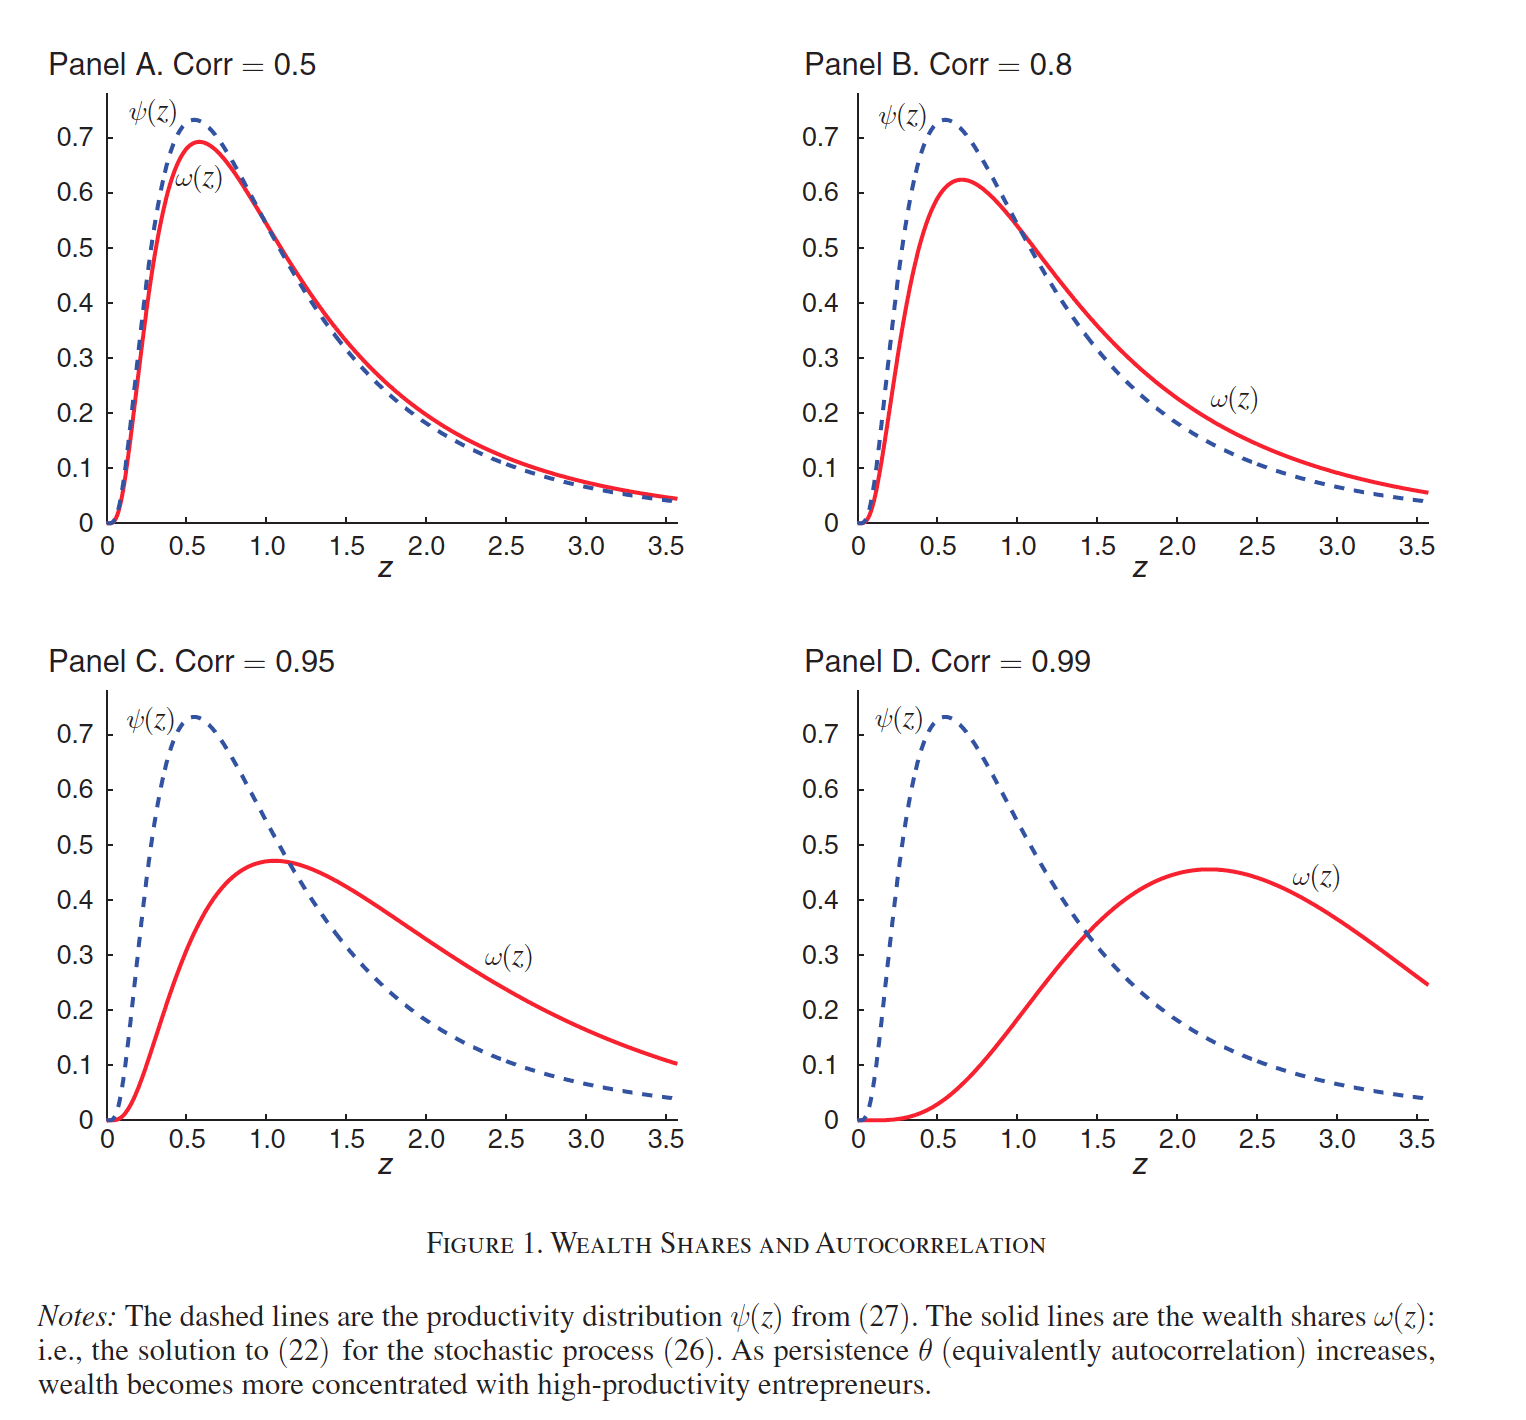
\includegraphics[scale=0.3]{figures/moll_1}
\end{figure}
\end{frame}

\begin{frame}{The importance of dynamics}
\begin{figure}
\centering
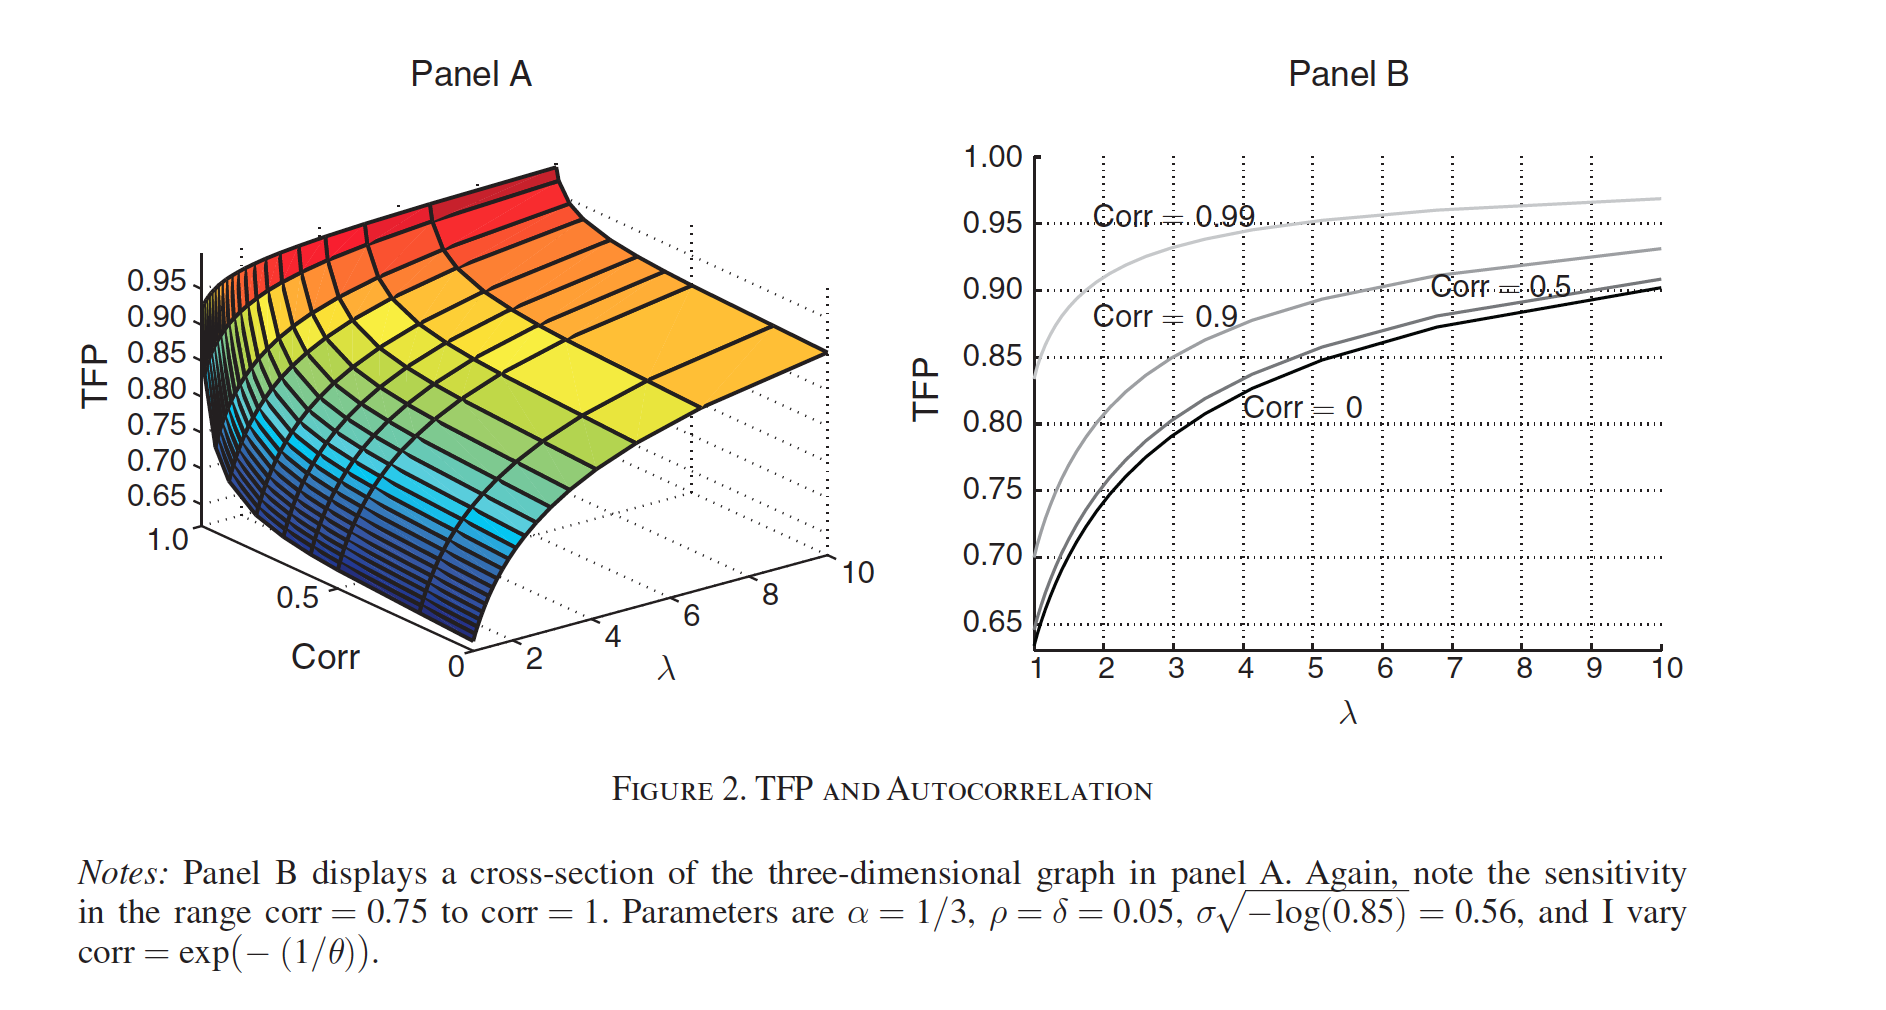
\includegraphics[scale=0.3]{figures/moll_2}
\end{figure}
\end{frame}


\begin{frame}{Transitional Dynamics}
\begin{itemize}
\item So far, effects comparing steady states
\item But after a reform that changes $\lambda$, how long should it take for economies to reach new steady state?
\item Insight: If $z$ is persistent, it can take a long time
\item Intuition: self-financing takes time
\end{itemize}
\end{frame}

\begin{frame}{The importance of dynamics}
\begin{figure}
\centering
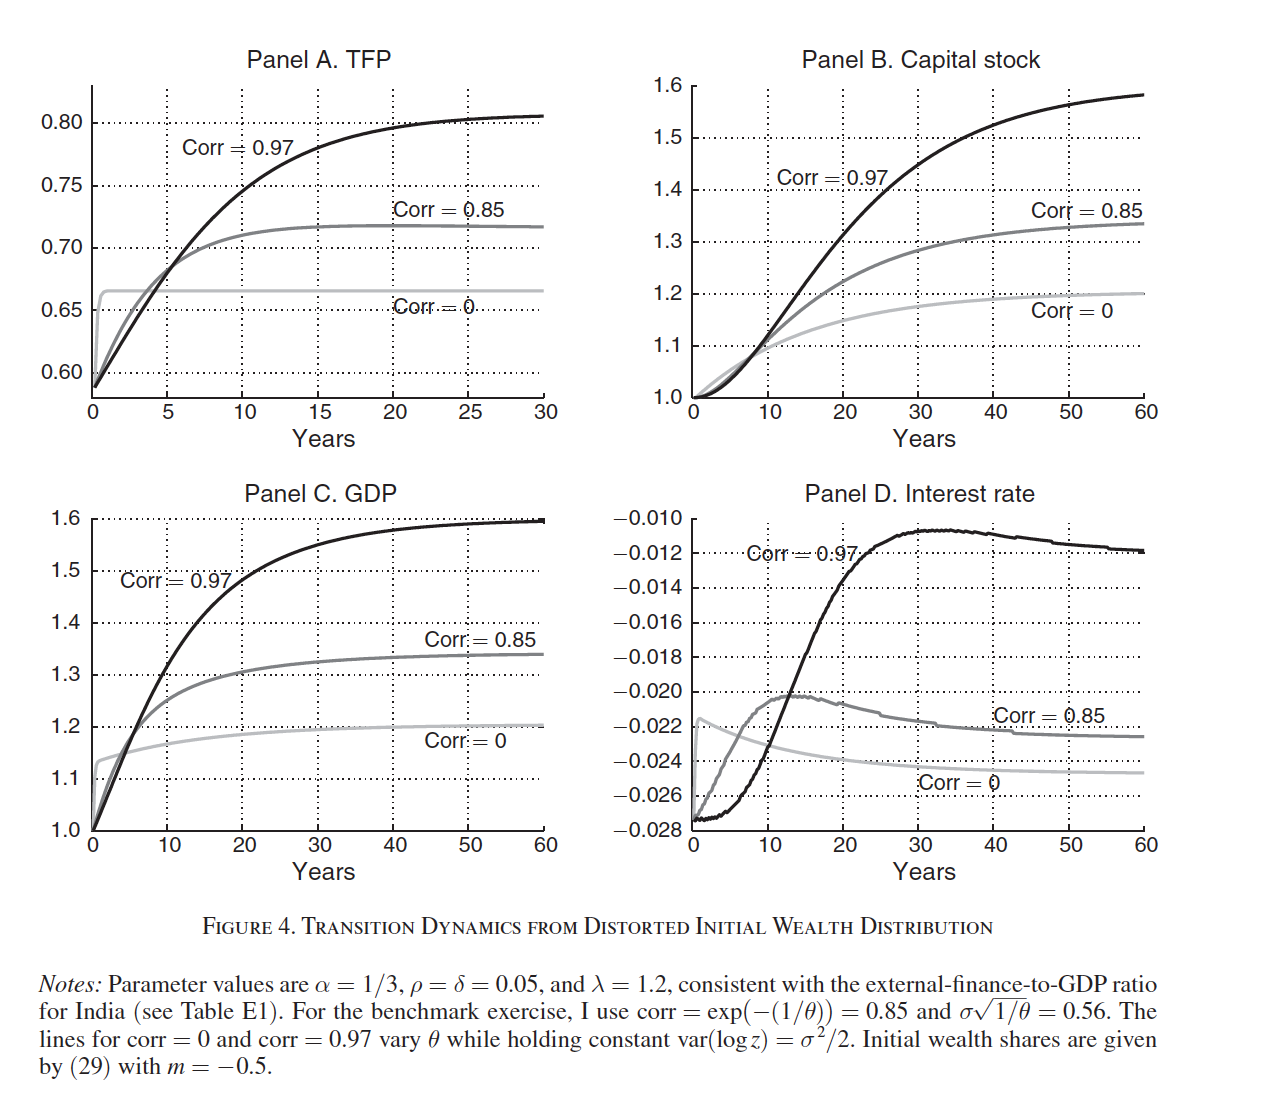
\includegraphics[scale=0.3]{figures/moll_6}
\end{figure}
\end{frame}

\begin{frame}
Several polar cases:

\begin{itemize}
\item Static model: Losses from financial frictions arbitrarily large
\item Steady State differences in Dynamic model
\begin{itemize}
\item i.i.d. firm-level productivity: arbitrarily large TFP losses, instantaneous transitions
\item Permanent firm level productivity: TFP losses go to zero, very long transitions
\end{itemize}
\item For realistic persistence
\begin{itemize}
	\item Meaningful steady-state losses, and transition dynamics take time
\end{itemize}
\end{itemize}
\end{frame}


\begin{frame}{The right persistence parameter}
Moll (2014) advocates persistence between 0.75 and 0.97 using evidence from Gourio (2008) and Asker, Collard-Wexler, and De Loecker (2014)
\begin{itemize}
\item Go back to figure 2 and discuss
\end{itemize}
\end{frame}

\begin{frame}{Moving Forward}
\begin{itemize}
\item Appeal of the model is its tractability
\item Perhaps unrealistic features
\begin{itemize}
\item Financial frictions matter not only for scale of production but entry/sectoral allocation
\item Decreasing returns to scale could be important. We are assuming the best firm can undertake the whole production of the economy
\item ...
\end{itemize}
\end{itemize}
\end{frame}
\end{document}



